\section{Functional Requirements}
\subsection{Introduction}

\subsubsection{Scope}
The \#YOCO utility should be implemented within the current AutoMart system and should not replace it. The subsystem needs to provide features that will help AutoMart reduce the number of poor and irrelevant advertisements on their website.

In this regard, the utility acts as a firewall that blocks bad quality images from entering the database while also validating that images that do pass as good quality, are well represented in the advertisement.

The system determines the image validity and quality by performing car detection, car coverage, blur and colour detection. Car detection is performed first as further tests and analysis require car location in the image in order to perform their own analysis. Car detection needs to check if the image contains a car. If the image contains a car, detection rating is set to one, and if no car is found detection rating is set to zero. Further tests are independent and can be conducted in any order. 

Car coverage calculates the area the car occupies in the image. Depending on the coverage percentage a value between zero and two is assigned to the coverage rating. Blur detection determines the image blurriness. Depending on the blurriness percentage a value between zero and two is assigned to the blur rating. Colour detection determines the colour of the car. AutoMart currently has sixteen colour buckets that are used to represent the colour of the car. The system calculate which colour bucket is the closest to the car's colour.

Finally the final image rating is calculated by adding detection rating, coverage rating and blur rating. The image rating and colour of the car are returned to the client side where further decisions can be performed based on clients preference. 

\pagebreak
\subsubsection{Limitations}
The system will not always be able to determine the correct colour of the car as aspects such as lighting, shadow and angle make it difficult to determine the colour correctly.

\subsubsection{Exclusions}
The system should only be implemented to work with cars and should not cater for the existence of any other vehicles such as motorcycles and trucks. The system is not able to determine the make and the model of the car. The recognition of different makes of the cars could be implemented in the future. However the recognition of models is not as no possible solution was found.

\subsection{Required Functionality}
\begin{figure}[h!]High Level Use Case Diagram.}
  \centering
	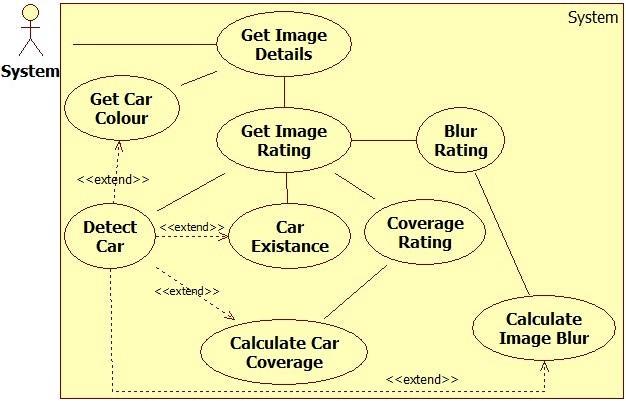
\includegraphics{HighLevelUseCase.jpg}
\end{figure}

\subsection{Use Cases}
\textbf{Detect Car Subsystem}\\
\begin{tabular}{ | l | l |}
	\hline
  	\multicolumn{2}{| c |}{\textbf{Find Bounding Box}} \\
  	\hline
  	\multicolumn{2}{| c |}{Determines if the car exists in the photo and returns co-ordinates of the box containing the car.}\\
	\hline
	Priority & Critical \\	
  	\hline
  	Pre-Conditions & A valid image needs to be provided.\\
  	\hline
 	Post-Conditions & Car detection status provided.\\
  	\hline
\end{tabular}\\
\\
\\
\textbf{Describe Car Subsystem}\\
\begin{tabular}{ | l | l | }
	\hline
  	\multicolumn{2}{| c |}{\textbf{Determine Colour}} \\
  	\hline
  	\multicolumn{2}{| c |}{Determines the colour of the car and finds the closest 3 colour buckets.}\\
	\hline
	Priority & Important \\	
  	\hline
  	Pre-Conditions & A car needs to exist in the bounding box.\\
  	\hline
 	Post-Conditions & Colour(s) of the car determined.\\
  	\hline
\end{tabular}\\
\\
\\
\begin{tabular}{ | l | l | }
	\hline
  	\multicolumn{2}{| c |}{\textbf{Calculate Blur}} \\
  	\hline
  	\multicolumn{2}{| c |}{Stretches the bounding box to 480x320 pixels and calculates and returns the blur value.}\\
	\hline
	Priority & Important \\	
  	\hline
  	Pre-Conditions & Bounding box exists.\\
  	\hline
 	Post-Conditions & Blur value successfully calculated and returned.\\
  	\hline
\end{tabular}\\
\\
\\
\begin{tabular}{ | l | l | }
	\hline
  	\multicolumn{2}{| c |}{\textbf{Calculate Coverage}} \\
  	\hline
  	\multicolumn{2}{| c |}{Calculates the coverage the car occupies in the photo.}\\
	\hline
	Priority & Important \\	
  	\hline
  	Pre-Conditions & Bounding box exists.\\
  	\hline
 	Post-Conditions & Car coverage  value successfully calculated and returned.\\
  	\hline
\end{tabular}\\
\\
\\
\pagebreak
\subsection{Process Specifications}
\begin{figure}[h!]
  \caption{Activity diagram of FindBoundingBox}
  \centering
	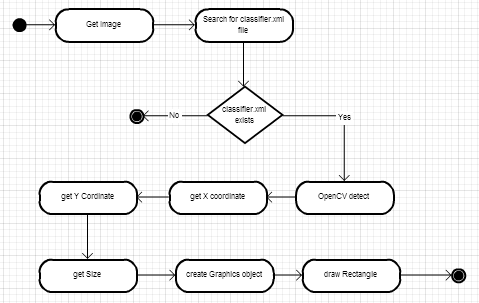
\includegraphics{activity.PNG}
\end{figure}
